%%%%%%%%%%%%%%%%%%%%%%%%%%%%%%%%%%%%%%%%%%%%%%%%%%%%%%%%%%%%%
%
% Section: Linear Functions and Their Slopes
%
%%%%%%%%%%%%%%%%%%%%%%%%%%%%%%%%%%%%%%%%%%%%%%%%%%%%%%%%%%%%%

\section{Linear Functions and Their Slopes}
\label{LinearFunctionsandSlope}

At the end of the last chapter, we took a look at functions in terms of their average rates of change, and noted that some functions have constant rates of change, while for others the rate of changes varies. We also noted that there is huge difference between these two types of functions.\\

In this chapter we will focus our attention on those special functions whose rates of change are always the same. We will see that there are actually rather a lot of useful functions which have this special property, and how knowing a function has a constant rate of change can help in setting up mathematical models.

%%%%%%%%%%%%%%%%%%%%%%%%%%%%%%%%%%%%%%%%%%%%%%%%%%%%%%%%%%%%%
%
% Subsection: Linear Functions and Their Slopes: Linear Functions and Slope
%
%%%%%%%%%%%%%%%%%%%%%%%%%%%%%%%%%%%%%%%%%%%%%%%%%%%%%%%%%%%%%

\subsection{Linear Functions and Slope}

We’ll begin by defining our terms:

\begin{definition}
	\index{Linear Function}
	\textbf{\underline{Definition Linear Function}}\\
	\bigskip
	A function is called \textbf{linear} if and only if it has a constant rate of change.\\
	The rate of change of a linear function is called its \textbf{slope}.
\end{definition}

In \ref{RatesofChange}, we looked at the average rates of change for various functions, and noted that for most functions, the rate of change is itself changing. For example, the rate of change for the distance you travel on a trip as a function of time is your speed, and your speed varies. So this would not be a linear function. Another example we considered was temperature as a function of time, and we noted the rate at which the temperature changes is not always the same, and so that would also not be a linear function.\\

On the other hand, we also looked at the amount of a residential electric bill as a function of the electricity used, and noted that it seemed reasonable that there would be a set cost per kilowatt-hour. If that is indeed true, that would mean that the amount of the bill as a function of electric usage has a constant rate of change, and therefore is a linear function.\\

If we have a linear function, knowing its constant rate of change (that is, its slope) would seem to be pretty useful information. How can we determine the slope? It turns out that we already know how! If everyone working for a company makes the same hourly rate, and the average wage is $\$12.50$ per hour, then logically it must be that everybody makes the same as the average -- $\$12.50$ per hour. By the same sort of logic, if a function always has the same rate of change, then that rate of change must be the same as the average rate of change. So, if a function is linear we can find its slope by finding its average rate of change.\\

Let’s make that official.

\begin{definition}
	\index{Linear Function!Slope}
	\textbf{\underline{Formula: The Slope of a Linear Function}}\\
	\bigskip
	The slope of a linear function can be found using the formula:\\
	\begin{equation*}
		slope = \frac{\Delta output}{\Delta input} = \frac{\Delta f(x)}{\Delta x}=\frac{f(b)-f(a)}{b-a}
	\end{equation*}
	where $a$ and $b$ are any two values in the domain of $f(x)$.
\end{definition}

An example will illustrate this formula’s use.

\exam{\label{LinearFunctionsandSlopeExample1} Suppose $f(x)$ is a linear function, and suppose $f(1)=3$ and $f(5)=27$. Find its slope.}

\indenttext{We have two input-output pairs for the function, so we can use them in the slope formula. If we choose $a=1$ and $b=5$, we get:
	\begin{align*}
		slope &= \frac{\Delta output}{\Delta input} = \frac{\Delta f(x)}{\Delta x}=\frac{f(b)-f(a)}{b-a}\\
		&\\
		&=\frac{f(5)-f(1)}{5-1}=\frac{27-3}{5-1}\\
		&\\
		&=\frac{24}{4}=6
	\end{align*}
	(We usually choose $a$ to be the smaller value, but we don’t have to. We’d have gotten the same result if we had let $a=5$ and $b=1$).
}

\bigskip

When calculating average rates of change we often got different averages depending on which input-output pairs we used. That happens with non-linear functions. But this is not an issue when calculating slope. Since the slope of a linear function is, by definition, a constant rate of change, it will come out to be the same regardless of which input-output pairs we use.

\exam{\label{LinearFunctionsandSlopeExample2} Suppose $g$ is a linear function, some of whose inputs and corresponding outputs are given in the following table. Find the slope.
	\begin{center}
		\begin{tabular}{c|c}
			t & g(t) \\
			\hline
			3 & 11 \\
			5 & 7 \\
			8 & 1
		\end{tabular}
	\end{center}
}

\indenttext{We have more input-output pairs than we actually need here. To use the formula we only need two. So we can choose any two to use. Using, say, $a=3$ and $b=8$ we get:
	\begin{align*}
		slope &= \frac{\Delta output}{\Delta input} = \frac{\Delta g(t)}{\Delta t}=\frac{g(b)-g(a)}{b-a}\\
		&\\
		&=\frac{g(8)-g(3)}{8-3}=\frac{1-11}{8-3}\\
		&\\
		&=\frac{-10}{5}=-2
	\end{align*}
	You can verify for yourself that choosing a different pair would give the same result.
}

\bigskip

While the formula for slope is essentially the same as the formula for average rate of change (AROC), it is important to distinguish between slope and AROC:

\begin{itemize}
	\item Every function has average rates of change. Only linear functions have slopes. The word \quotes{slope} should only be used if you know the function is linear.
	\item For linear functions, the average rate of change (AROC) and the slope are the same thing.  But for a non-linear function, this AROC is not a slope.  Again, the word \quotes{slope} should only be used with linear functions.
	\item  If a function is linear, it doesn’t matter which input-output pairs you use. The formula will always give the same value for the slope. But for non-linear functions, you may get different average rates of change depending on which input-output pairs you use.
\end{itemize}

%%%%%%%%%%%%%%%%%%%%%%%%%%%%%%%%%%%%%%%%%%%%%%%%%%%%%%%%%%%%%
%
% Subsection: Linear Functions and Their Slopes: Linear Functions and Mathematical Models
%
%%%%%%%%%%%%%%%%%%%%%%%%%%%%%%%%%%%%%%%%%%%%%%%%%%%%%%%%%%%%

\subsection{Linear Functions and Mathematical Models}

One of our main reasons for studying linear functions is that there are many real-world situations that can be modeled using them. Two of many possible examples are the following:

\exam{\label{LinearFunctionsandSlopeExample3}A contractor who refinishes hardwood floors calculates the prices, $p$, he quotes for jobs as a linear function of the area, $A$, in square feet to be refinished; call this function $h(A)$. For a job measuring $A=250$ square feet he charges $h(250)=500$ dollars. For a job measuring $A=600$ square feet he charges $h(600)=1025$ dollars. What is the slope of this pricing function $h(A)$? What is the rate at which he changes prices based on area?}

\indenttext{
	The function is linear so we can calculate its slope:

	\begin{equation*}
		slope = \frac{\Delta output}{\Delta input} =\frac{h(600)-h(250)}{600-2500} = \frac{1025-500}{600-250} = \frac{525}{350}=1.5\\
	\end{equation*}

	So, the slope is $1.5$.\\
	\newline

	The rate of change here is the slope. The units of a rate of change are always \quotes{output units per input unit}, and so since the output units are dollars and the input units are square feet, the rate of change is $\$1.50$ per square foot. In other words, for each additional square foot of area, he raises the price of the job by $\$1.50$.
}

\exam{\label{LinearFunctionsandSlopeExample4} The scientist Galileo Galilei (1564-1642) discovered the principle of \quotes{uniform acceleration} -- that the speed at which a dropped object travels is a linear function of the time since it was dropped.  Suppose that at time $t=0$ the speed of a dropped rock is $v(0)=0$ feet per second, and after $2.5$ seconds its speed is $v(2.5)=80$ feet per second. What is the slope of the function $v(t)$?  What is the rate of change of the rock’s velocity?
}

\indenttext{Since we know the function is linear we can calculate its slope:

	\begin{equation*}
		slope = \frac{\Delta output}{\Delta input} =\frac{v(2.5)-v(0)}{2.5-0} = \frac{80-0}{2.5-0}=32\\	
	\end{equation*}

	So the slope of this function is 32.\\
	\newline

	The rate of change of velocity is the slope of the velocity function, but to answer the question asked we should include units in the answer. Remember that the units of an average rate of change (and therefore the units of a slope) are always \quotes{output units per input unit}, so the rate of change of the rock’s velocity would be 32 feet per second per second.
}

\bigskip

Now, in all of the examples we’ve considered so far, we’ve known the function was linear because the problem specifically said it was linear. But could we have known that without specifically being told? Surely the contractor knows that he’s pricing jobs using a rate of $\$1.50$ per square foot, but it’s not at all certain that he knows that he’s using the slope of a linear function. And we know for certain that Galileo wasn’t thinking about linear functions when he was studying the speed at which objects fall – because the concept of a \quotes{linear function} did not exist until long after his death!  How did anyone ever determine that these functions were linear?\\

The key to knowing whether or not a given situation can be mathematically modeled with a linear function is to ask \quotes{does this function have a constant rate of change.} So, we need to think about the average rate of change and what it means in terms of the situation given, and then ask whether or not that average rate of change would always be the same.\\

So, in the case of the contractor, price is a function of the area to be refinished. So price is the output, and area is the input, and so the average rate of change would be how much price changes as the area to be refinished changes, and it would be measured in dollars per square foot. Does the contractor change his price per square foot (perhaps giving discounts for larger jobs), or does he increase his overall job price based on the area based on the same per-square-foot cost? If - and only if - the overall job cost changes at the same rate based on the area, then it is a linear function.\\
Likewise, if - and only if - the speed of the falling rock is always changing at the same rate, then speed is a linear function of time. Galileo’s observation of \quotes{uniform acceleration} means that, yes, the speed always changes at the same rate, and so the function is indeed linear.
\footnote{Actually this is not quite correct. The force of gravity grows stronger the closer you get to the center of the earth, and so as the rock falls the rate at which its speed accelerates actually does change very slightly. However, this change in acceleration is extremely slight and so it is generally ignored. This means a linear function is not perfectly accurate, but is good enough for almost any reasonable purpose.}\\

A few examples will illustrate how this works.

\exam{\label{LinearFunctionsandSlopeExample5} An auto insurance company determines its rates for a policy based on the number of points you have on your license. They start with a base rate of $\$600$ which you would pay regardless of how many points you have, and then they add a fixed dollar surcharge of $\$80$ for each point. Your insurance rate is a function of how many points you have. Is it a linear function?
}

\indenttext{Your insurance rate changes as the number of points you have on your license changes, and following the \quotes{output units per input unit} model this rate of change would be measured in dollars per point. From the description it is clear that this rate of change is a constant $\$80$ per point, and so the function is indeed linear. In fact, we know that $\$80$ per point is its slope.
}

\exam{\label{LinearFunctionsandSlopeExample6} Cattarauqua Ginseng Enterprises sells wholesale premium grade American ginseng at a price of $\$18$ per pound for the first $100$ pounds, and then each additional pound over $100$ pounds costs $\$16$. Cost is a function of weight. Is it a linear function?
}

\indenttext{The rate of change would be how quickly the price of your order rises as its weight increases, measured in dollars per pound. As you add additional pounds to your order, the price rises at a rate of $\$18$ per pound. But, once you reach $100$ pounds, the price then rises at a rate of $\$16$ per pound. So the rate of change itself changes. So this function is not linear.
}

\exam{\label{LinearFunctionsandSlopeExample7} A landscaper needs to determine the amount of fertilizer to load into a spreader to fertilize a town’s athletic fields. All the fields have the same type of terrain and are planted with the same type of grass. The amount of fertilizer needed (in pounds) is a function of the area to be covered (in square yards). Is it a linear function?
}

\indenttext{We need to consider the rate at which the amount of fertilizer changes as the area to be covered increases, measured in pounds per square yard. So we are talking about an application rate for the fertilizer. Based on the information given, it would seem that there would be a constant rate of application for the fertilizer, so, yes, this is almost certainly a linear function.
}

\exam{\label{LinearFunctionsandSlopeExample8} The circulation manager for a public library is keeping records about the total number of books checked out at any given time, beginning at the start of 2011. The number of books checked out of the library is a function of time since the start of the year. Is it a linear function?
}

\indenttext{The number of books checked out at any given time is of course changing, and its rate of change would be measured in books per day. (We are assuming time would be measured in days, though it could also be measured in hours or weeks or minutes too, but that doesn’t affect our problem here.) So, would the library always see the number of books checked out changing at the same rate of books per day? That seems absurdly unlikely. This function cannot possibly be linear.
}

\bigskip

In the exercises you’ll have the opportunity to work through some more examples, and we will see even more about this as we continue through the rest of the chapter. At first you will probably need to think things through slowly and carefully, but with practice you will find it becomes much easier to identify whether or not a linear function suits a given modeling situation.

%%%%%%%%%%%%%%%%%%%%%%%%%%%%%%%%%%%%%%%%%%%%%%%%%%%%%%%%%%%%%
%
% Subsection: Linear Functions and Their Slopes: Graphs of Linear Functions
%
%%%%%%%%%%%%%%%%%%%%%%%%%%%%%%%%%%%%%%%%%%%%%%%%%%%%%%%%%%%%

\subsection{Graphs of Linear Functions}

The name \quotes{linear} suggests something to do with lines, and the word \quotes{slope} suggests something to do with steepness. This is not a coincidence. In fact, these names are suggestive of what we can expect from the graphs of functions whose rates of change are constant.\\

Let’s consider a simple example of a linear function. Suppose water is flowing into a tub at a steady rate of 2 gallons per minute. Then the amount of water in the tub is a function of time since the faucet was turned on, and it is a linear function since its rate of change is a constant 2 gallons per minute, as long as we only include in our function’s domain the time that water is actually flowing (i.e. we don’t consider the time before the faucet is turned on or after the tub is full).  Suppose we call this function $f(t)$. We can create a table that shows how much water is in the tub at certain times:

\begin{center}
	\begin{tabular}{c|c}
		$t$ (minutes) & $f(t)$ (gallons) \\
		\hline
		0 & 0 \\
		1 & 2 \\
		2 & 4 \\
		3 & 6 \\
		4 & 8 \\
	\end{tabular}
\end{center}

Now, if we plot the points in the coordinate plane, we see that they fall in a straight line (we’ve chosen the window to show the portion of the coordinate plane where all of our points fall):

\begin{figure}[H]
	\centering
	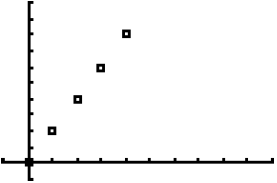
\includegraphics[scale=1.0]{Sections/LinearFunctionsandSlopeImages/Figure01.png}
	\caption{A plot of the values in the table}
\end{figure}

Is this a coincidence? Does it just look like a straight line for the particular points we happened to pick? Might the graph actually swerve upward or downward or flatten out if we look at the whole picture instead of just a few points?\\

This is not a coincidence at all, and actually the fact that the rate of change is constant makes it absolutely necessary that the function’s graph be a straight line. Remember that:

\begin{equation*}
	slope = \frac{\Delta output}{\Delta input}
\end{equation*}

Now, since the vertical axis is the output axis, changes in output show up in the graph as vertical changes, or in other words, up or down movement of the graph. We call the up-down movement in the graph its \textbf{rise}. By the same token, the horizontal axis is the input axis, and changes in input show up as horizontal changes, or right or left movement of the graph. We call this right or left movement \textbf{run}. So, putting this together with the definition of slope, we get:

\begin{equation*}
	slope = \frac{\Delta output}{\Delta input}=\frac{vertical \text{ } change}{horizontal \text{ } change} = \frac{rise}{run}
\end{equation*}

Suppose we zoom in and look at our filling-tub function’s graph between, say, $t=1$ and $t=2$.  Between these points the input changes by $2-1=1$ minute. And the output changes by $4-2=2$ gallons. We can see this in the graph as a rise of 2 and a run of 1:

\begin{figure}[H]
	\centering
	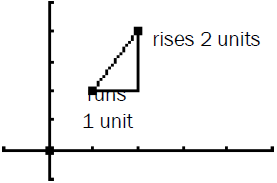
\includegraphics[scale=1.0]{Sections/LinearFunctionsandSlopeImages/Figure02.png}
	\caption{Visualizing slope graphically}
\end{figure}

We can see the same thing if we look, say, between $t=0$ and $t=3$. The run is 3 minutes, and the rise is 6 gallons, keeping the slope where it should be at 6 = 2 gallons per minute.\\

The slope shows up in the graph as steepness. The slope is a constant 2, and so the graph rises with a constant steepness of rising 2 units per 1 unit of run. Since the slope never changes, the steepness never changes, and so we cannot possibly end up with anything other than a straight line graph for the function overall:

\begin{figure}[H]
	\centering
	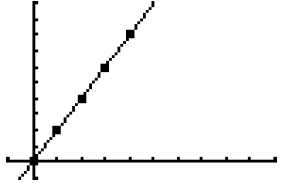
\includegraphics[scale=1.0]{Sections/LinearFunctionsandSlopeImages/Figure03.png}
	\caption{Graph of water in tub vs. time}
\end{figure}

In summary: Slope shows up in a graph as steepness. Because slope is constant, a linear function’s graph must have constant steepness, And so, a function is linear if and only if its graph is a straight line.

\exam{\label{LinearFunctionsandSlopeExample9}The height of a sunflower is a function of time since the seed was planted. This function is sketched in the graph below.
	\begin{figure}[H]
		\centering
		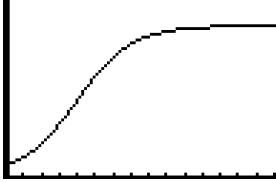
\includegraphics[scale=1.0]{Sections/LinearFunctionsandSlopeImages/Figure04.png}
		\caption{Graph of water in tub vs. time}
	\end{figure}
	\noindent Could this be a linear function? How do you know?
}

\indenttext{If the function were linear, its graph would be a straight line. This graph is not. The steepness of the graph changes, reflecting the fact that the plant grows more rapidly at certain times of its life cycle than at others. Because the steepness and the rate of growth that it represents are not constant, the function cannot possibly be linear.
}

\bigskip

The steepness of a graph indicates its rate of change. If a function has a very large rate of change, the graph will be very steep. If a function has a slow rate of change, the graph will be flatter.\\

If the function is increasing, the slope will be positive and the graph will slope upward. If the function is decreasing, the slope will be negative, and the graph will slope downward.

\exam{\label{LinearFunctionsandSlopeExample10} Four graphs are shown in the window below. Each graph belongs to a function which gives the amount of water in a family pool (in gallons) as a function of time (in minutes). All four pools start out with 500 gallons of water.\\

	The Ahmed’s are filling their pool at a steady rate of 20 gallons per hour.\\
	The Billigsley’s are draining their pool at a steady rate of 20 gallons per hour.\\
	The Chao’s are filling their pool at a steady rate of 50 gallons per hour.\\
	The Damiani’s aren’t doing anything.\\

	Which graph goes with which family’s pool?
	\begin{figure}[H]
		\centering
		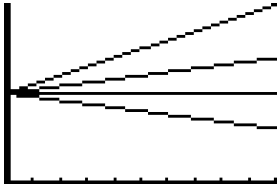
\includegraphics[scale=1.0]{Sections/LinearFunctionsandSlopeImages/Figure05.png}
	\end{figure}
}

\indenttext{The Billingsley’s are draining their pool, so the amount of water in their pool is decreasing as a function of time. So theirs must be the downward sloping line.\\

	The Ahmed’s and the Chao’s are both filling their pools, so they must own the rising lines. Since the Chao’s are filling their pool faster, their slope is larger, and so their graph must be the steeper one.\\

	Since the Damiani’s aren’t doing anything, their slope is zero and their graph must be the flat one.
}

\bigskip

We have seen that we can find the slope of a given function based on knowing any two of its input-output pairs. Input-output pairs are the points on the graph of the function. And so, if we know any two points on a linear function’s graph, we can calculate the function’s slope.

\exam{\label{LinearFunctionsandSlopeExample11} Find the slope of the linear function whose graph passes through the points $(3,5)$ and $(-4,13)$.}

\indenttext{We have two input values to use. Suppose we take them in the order given and say $a=3$ and $b=-4$. (It doesn’t matter which you call $a$ and which you call $b$; everything works out fine whichever you choose.) Following the formula we get:
	\begin{equation*}
		slope=\frac{\Delta output}{\Delta input} = \frac{\Delta f(x)}{\Delta x} = \frac{f(-4)-f(3)}{-4-3}=\frac{13-5}{-4-3}=\frac{8}{-7}
	\end{equation*}
	So the slope is $-\frac{8}{7}$.
}

\bigskip

Sometimes the slope formula is written differently, based on the idea of using two points on the graph to determine slope. If we have two points, which we call $(x_1,y_1)$ and $x_2,y_2)$ we can use the formula:

\begin{equation*}
	slope=\frac{y_2-y_1}{x_2-x_1}
\end{equation*}

It’s likely that you’ve seen the slope formula written in this way at some point in the past. While this formula is correct and it works just fine, it really isn’t necessary. It’s really just another way of writing the slope formula that we’ve been using.\\

In this text, we’ll continue to use the function-notation formula for slope we’ve been using. There really is no advantage to this other two-point formula, and the function-notation formula we’ve been using is both more general and also will prove more useful to you in your future mathematical career. So, while it is not incorrect to use this other formula if you are used to using it, it is probably going to be to your advantage to try to stick with the function-notation formula we’ve been using.

%%%%%%%%%%%%%%%%%%%%%%%%%%%%%%%%%%%%%%%%%%%%%%%%%%%%%%%%%%%%
%
% Subsection: Linear Functions and Slope: Exercises
%
%%%%%%%%%%%%%%%%%%%%%%%%%%%%%%%%%%%%%%%%%%%%%%%%%%%%%%%%%%%%

\clearpage

\subsection{Exercises}

\subsubsection*{Linear Functions and Slope}
Where necessary, either express your answers as a reduced fraction or a decimal rounded to two decimal places.

\bigskip	
\ex{$f(x)$ is a linear function, and $f(2) = 7$ and $f(4) = 13$. Find its slope.}
\sol{$3$}

\bigskip	
\ex{$f(x)$ is a linear function, and $f(3) = 9$ and $f(4) = 16$. Find its slope.}

\bigskip	
\ex{$g(x)$ is a linear function, and $g(40) = 70$ and $g(90) = 10$. Find its slope.}
\sol{$-\frac{6}{5}=-1.2$}

\bigskip	
\ex{$g(x)$ is a linear function, and $g(800) = 2200$ and $g(100) = 900$. Find its slope.}

\bigskip	
\ex{$f(t)$ is linear, $f(-4) = 8$ and $f(1) = -11$. Find the slope of $f(t)$.}
\sol{$-\frac{19}{5}=-3.8$}

\bigskip	
\ex{$h(x)$ is linear, $h(-1) = 5$ and $h(3) = -17$. Find the slope of $h(x)$.}

\bigskip	
\ex{$w(-3) = -1$, $w(-9) = 15$, and $w(z)$ is a linear function. Find its slope.}
\sol{$-\frac{8}{3}=-2.67$}

\bigskip	
\ex{$f(-2) = -7$, $f(-10) = -16$, and $f(w)$ is linear. Find its slope.}

\bigskip	
\ex{$f(x)$ is linear. $f(3) = 11$, $f(2) = 6$, and $f(0) = -4$. What is the slope of $f(x)$?}
\sol{$5$}

\bigskip	
\ex{Suppose $g(x)$ is linear and the table below contains inputs and outputs for $g(x)$. Find the function’s slope.	
	\begin{center}
		\begin{tabular}{|c|c|}
			\hline
			$x$ & $g(x)$ \\
			\hline
			5 & 8825 \\
			\hline
			12 & 3680 \\
			\hline
			27 & -7345 \\
			\hline
		\end{tabular}
	\end{center}	
}

\bigskip	
\ex{Suppose the table shown below contains some input-output pairs for the linear function $f(x)$. Determine the function’s slope.
	\begin{center}	
		\begin{tabular}{|c|c|c|c|c|}
			\hline
			$x$ & 800 & 1200 & 15,000 & 0 \\
			\hline
			$f(x)$ & 21.7 & 9.7 & -404.3 & 45.7 \\
			\hline
		\end{tabular}
	\end{center}
}	
\sol{$-\frac{3}{100}=0.03$}


\bigskip	
\ex{$p(0) = 12$, $p(16) = 68$, $p(32) = 124$, and $p(5) = 29.5$. $p(x)$ is linear. What is its slope?}
\bigskip	

\subsubsection*{Linear Functions and Mathematical Models}

\bigskip	
\ex{Kilgore Trout’s Literary Review pays published authors based on the length of the stories published. The amount paid is a linear function of the number of words. For a story of $w = 1850$ words the review pays $p(1850) = 200$ dollars. For a $w = 2350$ word story, they pay $p(2350) = 250$ dollars. Find the slope of this function, and interpret its meaning (including units.)}
\sol{$\frac{1}{10}=0.1$, units are dollars per word so this is best written as $\$0.10/word$.  This represents how much the amount that they pay changes based on the number of words in the article, or, in more common terms, how much they pay per word.}

\bigskip	
\ex{Stuckeybowl Lanes hosts bowling birthday parties for children. The charge for a birthday party is a linear function of the number of children attending. For $x = 9$ kids the cost is $p(9) = 223.35$ dollars. For $x = 17$ kids the cost is $p(17) = 382.95$ dollars. Find the slope of this function, and interpret its meaning (including units).}

\bigskip	
\ex{Fire safety codes specify the maximum number of people who can safely occupy a building or room at a given time. You’ve probably seen signs in public areas stating the maximum occupancy allowed. The maximum number of occupants allowed is a function of the area.  According to the Life Safety Code, the maximum number of allowed occupants is one person for each five square feet if the overall area is less than 10,000 square feet, and one person for every seven square feet if the overall area is greater than 10,000 square feet. Is maximum occupancy a linear function of area? Justify your answer.}
\sol{No, it is not a linear function.  The rate of change is not always the same; sometimes in this 1/5 person per square foot and sometimes it is 1/7 person per square foot.  A linear function must always have the same rate of change.}

\bigskip	
\ex{An architect is designing a church and needs to determine the amount of pew space needed. The total required length of the pews is a function of the planned maximum occupancy of the church, and building codes specify that there must be 18 inches of pew space per person. Is required pew space a linear function of planned maximum occupancy? Justify your answer.}

\bigskip	
\ex{A banquet manager determines the amount of baked ziti to prepare based on the number of guests expected to attend. Would it be reasonable to expect the amount of ziti to prepare to be a linear function of the number of expected guests? Justify your answer.}
\sol{Yes, it would be reasonable to plan for a certain amount of food per person.  There is no reason to think the amount the average person would eat based on the number of people invited.}

\bigskip	
\ex{The plant manager for the Stuckeyville Pure Waters plant monitors the amount of water in the town reservoir over time. Would it be reasonable to expect the amount of water in the reservoir to be a linear function of time since the start of the year? Justify your answer.}

\bigskip	
\ex{In the State of Michigan, the amount of state income tax owed is a function of taxable income. The tax rate is a flat $5.3\%$ of taxable income. Is the amount of Michigan state income tax a linear function of taxable income? Justify your answer.}
\sol{Yes, it is linear.  The amount your tax changes as your income increases is always $\$0.053$ tax per dollar or income.}

\bigskip	
\ex{In the State of New York, the amount of state income tax owed is a function of taxable income. The tax rate varies between $4.0\%$ and $8.97\%$, with those making higher incomes paying a higher rate than those who earn less. Is the amount of New York state income tax a linear function of taxable income? Justify your answer.}

\bigskip	
\ex{An urban planner is studying population changes in Las Vegas, Nevada and has collected data giving the city’s population as a function of time (in years) since 1950. Is it reasonable to think that this function is linear? Justify your answer.}
\sol{No, it is not.  The population of a city would not be expected to always change at the same rate of number of people per year. }

\bigskip	
\ex{An industrial economist is studying the projected total installed capacity of Chinese nuclear power plants over the next 50 years. The Chinese government has stated its intention to carefully regulate the growth of this installed capacity so that it grows at a steady rate. Would it be reasonable for the economist to treat the projected installed nuclear capacity as a linear function of time? Justify your answer.}

\bigskip	
\subsubsection*{Graphs of Linear Functions}

\bigskip	
\ex{Which of the following could be graphs of linear functions? Justify your answers.
	\begin{tasks}(2)
		\task[a.] \begin{figure}[H] 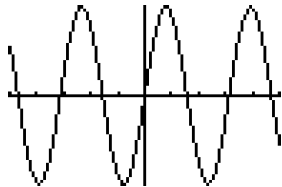
\includegraphics[scale=1.0]{Sections/LinearFunctionsandSlopeImages/Exercise23a.png} \end{figure}
		\task[b.] \begin{figure}[H] 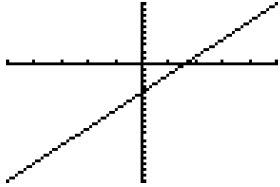
\includegraphics[scale=1.0]{Sections/LinearFunctionsandSlopeImages/Exercise23b.png} \end{figure}
		\task[c.] \begin{figure}[H] 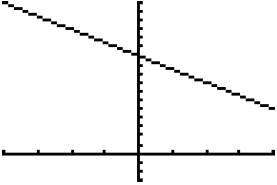
\includegraphics[scale=1.0]{Sections/LinearFunctionsandSlopeImages/Exercise23c.png} \end{figure}
		\task[d.] \begin{figure}[H] 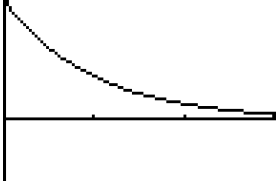
\includegraphics[scale=1.0]{Sections/LinearFunctionsandSlopeImages/Exercise23d.png} \end{figure}
	\end{tasks}
}
\sol{a. could not be, the graph is clearly not a straight line.\\
	b. could be, the graph appears to be a straight line.\\
	c. could be, the graph appears to be a straight line.\\
	d. could not be, the graph is clearly not a straight line.}

\bigskip	
\ex{Which of the following could be graphs of linear functions? Justify your answers.
	\begin{tasks}(2)
		\task[a.] \begin{figure}[H] 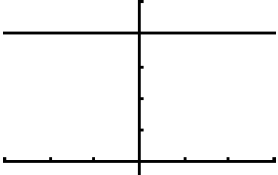
\includegraphics[scale=1.0]{Sections/LinearFunctionsandSlopeImages/Exercise24a.png} \end{figure}
		\task[b.] \begin{figure}[H] 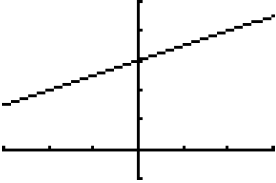
\includegraphics[scale=1.0]{Sections/LinearFunctionsandSlopeImages/Exercise24b.png} \end{figure}
		\task[c.] \begin{figure}[H] 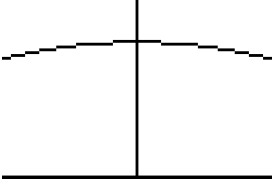
\includegraphics[scale=1.0]{Sections/LinearFunctionsandSlopeImages/Exercise24c.png} \end{figure}
		\task[d.] \begin{figure}[H] 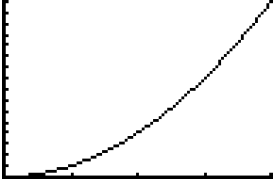
\includegraphics[scale=1.0]{Sections/LinearFunctionsandSlopeImages/Exercise24d.png} \end{figure}
	\end{tasks}
}
\bigskip
25-38: if the answer is not a whole number, express your answer either as a decimal (rounded to two decimal places as needed) or a reduced fraction.
\bigskip	
\ex{Find the slope of the linear function whose graph passes through the points $(0,2)$ and $(3,14)$.}
\sol{$4$}

\bigskip	
\ex{Find the slope of the linear function whose graph passes through the points $(5,7)$ and $(11,49)$.}

\bigskip	
\ex{What is the slope of the linear function whose graph passes through the points $(-3,1)$ and $(2, -9)$?}
\sol{$-2$}

\bigskip	
\ex{What is the slope of the linear function whose graph passes through the points $(-4, -9)$ and $(-1, -25)$.}

\bigskip	
\ex{The graph of a given function is a straight line which passes through the points $(5, -3)$ and $(-3,5)$. What is the function’s slope?}
\sol{$-1$}

\bigskip	
\ex{The graph of $f(x)$ is a straight line which passes through the points $(-2,11)$ and $(2, -11)$. What is the slope of $f(x)$?}

\bigskip	
\ex{Determine the slope of the linear function whose graph passes through the points $(-3, -8)$ and $(-6, -15)$.}
\sol{$\frac{7}{3}=2.33$}

\bigskip	
\ex{Determine the slope of the linear function whose graph passes through the points $(-2000, 3500)$ and $(-2300, -4875)$.}

\bigskip	
\ex{A linear function’s graph passes through the points $(107,429)$ and $(338, -219)$. What is the function’s slope?}
\sol{$-\frac{216}{77}=-2.81$}

\bigskip	
\ex{A linear function’s graph passes through the points $(17,41)$ and $(23, -11)$. What is the function’s slope?}

\bigskip	
\ex{What would be the slope of a linear function whose graph passes through the points $(\frac{-7}{4},\frac{2}{3})$ and $(\frac{3}{5},\frac{-5}{8})$?}
\sol{$-\frac{155}{282}=0.55$}

\bigskip	
\ex{What would be the slope of a linear function whose graph passes through the points $(\frac{32}{5},\frac{2}{9})$ and $(\frac{-118}{25},\frac{-17}{3})$?}

\bigskip	
\ex{What is the slope of the linear function whose graph passes through $(2,8)$ and $(17,8)$?}
\sol{$0$}

\bigskip	
\ex{What is the slope of the linear function whose graph passes through $(4, -3)$ and $(-1, -3)$?}

\bigskip	
\ex{In questions 25-37 odd, which of the linear functions are increasing, which are decreasing, and which are constant? How do you know? }
\sol{If a linear function is increasing, then the slope is positive.  So, \#25 and \#31 are increasing linear functions.\\
	If a linear function is decreasing, then the slope is negative.  So, \#27, \#29, \#33 and \#35 are decreasing linear functions.\\
	If a function is constant, it is not changing (neither increasing nor decreasing), so it's slope is zero which is \#37.}

\bigskip	
\ex{In questions 26-38 even, which of the linear functions are increasing, which are decreasing, and which are constant? How do you know? }

\bigskip	
\ex{\begin{enumerate}[label=(\alph*)]
		\item Find the slope of the linear function whose graph passes through (2,11) and (2,5).
		\item Why is this a trick question?
\end{enumerate} }
\sol{a.  cannot, it requires division by zero which is impossible.\\
	b.  A line which passes through those points would be vertical, and so it would by its very nature fail to be a function.}

\bigskip	
\ex{This is a trick question. Suppose $f(5) = 7$ and $f(8) = 3$. What is the slope of $f(x)$? }

\bigskip	
\subsubsection*{Grab Bag}

\bigskip	
\ex{Suppose I’ve used my graphing calculator to create a table for the linear function $w(t)$.  The results are shown below.  What is the function’s slope?\\
	\begin{figure}[H] \centering 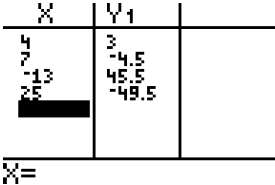
\includegraphics[scale=1.0]{Sections/LinearFunctionsandSlopeImages/Exercise43.png} \end{figure}
}
\sol{$-2.5$}

\bigskip	
\ex{Could the table below have been created using a linear function? How do you know?\\
	\begin{figure}[H] \centering 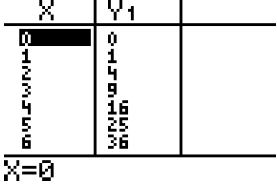
\includegraphics[scale=1.0]{Sections/LinearFunctionsandSlopeImages/Exercise44.png} \end{figure}
}

\bigskip	
\ex{Could the table below have been created using a linear function? How do you know?\\
	\begin{figure}[H] \centering 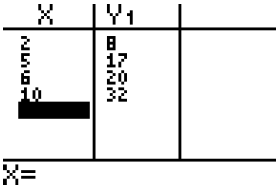
\includegraphics[scale=1.0]{Sections/LinearFunctionsandSlopeImages/Exercise45.png} \end{figure}
}
\sol{Yes, it could be.  The output (Y) values increase by 3 for every 1 unit that the input (X) values increase by, so this could be from a linear function with a slope of 3.  (We cannot say for sure because we only have these three points; the average rate of change might be different for this function for points that didn't happen to ve included in the table.  So all we can say is that this could be linear.)}

\bigskip	
\ex{Let $P(t)$ be the population of the world $t$ years from right now. Is $P(t)$ a function? Is $P(t)$ a linear function? Explain your reasoning. }

\bigskip	
\ex{Temperature in degrees Fahrenheit is a linear function of temperature in degrees Celsius.  The freezing point of water is $32^\circ$F or $0^\circ$C. The boiling point of water is $212^\circ$F or $100^\circ$C. What is the slope of this function? }
\sol{$frac{9^\circ \text{F}}{5^\circ \text{C}}=1.8 \frac{^\circ \text{F}}{^\circ \text{C}}$}

\bigskip	
\ex{Temperature in degrees Celsius is a linear function of temperature in degrees Fahrenheit.  The freezing point of water is $32^\circ$F or $0^\circ$C. The boiling point of water is $212^\circ$F or $100^\circ$C. What is the slope of this function? }

\bigskip	
\ex{The function $f(x) = 50 - 3x$ is a linear function. Choose any two values for $x$ and find the corresponding values for $f(x)$. Then, use those two input-output pairs to determine the slope of this function. }
\sol{$3$}

\bigskip	
\ex{Find the slope of the linear function whose graph passes through $(\frac{2}{3},\frac{3}{8})$ and $(-\frac{4}{5},-\frac{7}{3})$?}

\bigskip	
\ex{Suppose $h(t)$ is linear, $h(25) = 9,800$ and $h(40) = 11,000$. What is the slope of $h(t)$? }
\sol{$80$}

\bigskip	
\ex{A bread recipe calls for 2 cups of flour and 3 teaspoons of yeast. It also says \quotes{this recipe can be adjusted to make a larger batch; for each additional cup of flour add one additional teaspoon of yeast}. The amount of yeast is a function of the amount of flour. Is it a linear function? If so, what is its slope (include units in your answer)? If not, clearly explain why not. }

\bigskip	
\ex{A screen printer produces custom T-shirts to order. The company brochure states that the standard minimum order is 50 shirts for which the charge is \$175. The brochure also states that \quotes{for larger orders, add \$50 for each 25 additional shirts}.
	\begin{enumerate}[label=(\alph*)]
		\item The cost of an order is a function of the number of shirts ordered above the minimum order. Is it a linear function? If so, what its slope (include units in your answer)? If not, clearly explain why not. 
		\item Is the cost of an order a linear function of the number of shirts ordered? Why or why not? 
	\end{enumerate}
}
\sol{a.  Yes, it is a linear function.  The slope is \$2 per additional shirt.  (This answer makes the natural assumption that the domain of the function only includes positive numbers.\\
	b.  No, it is not a linear function.  Not ordering any shirts would cost \$0, byt ordering 50 shirts costs \$175.  So the average rate of change between 0 and 50 shirts is \$3.50 per shirt.  However, increasing the order beyond that the average rate of change is \$2 per shirt.  Since the average rate of change is not always the same, the function is not a linear function.)}

\bigskip	
\ex{An online merchant charges a standard minimum shipping charge of \$7.95 for orders \$50 and under. For orders between \$50 and \$125 the shipping charge is \$9.95 and for orders \$125 and over the charge is \$11.95. Shipping charge is a function of the amount of merchandise ordered. Is it a linear function? If so, what is its slope (include units in your answer)? If not, clearly explain why not. }

\bigskip	
\ex{A trucking company guarantees delivery time based on the number of miles a shipment must travel. For a shipment going up to 600 miles, the guaranteed delivery based on a rate of 1 hour for every 50 miles. For shipments going more than 600 miles, the company adds in an additional 8 hours for each 300 miles to allow for a rest break for the driver. Guaranteed delivery time is a function of distance. Is it a linear function? If so, what is its slope (include units in your answer)? If not, clearly explain why not.}
\sol{It is not a linear function.  Up to 600 miles, the average rate of change is 1/50 hour per mile.  Above 600 miles the average rate of change is 2/75 hours per mile.  Since these are not the same, the function is not a linear function.}

\bigskip	
\ex{Let $d(t)$ be the depth of water in a tidal pool $t$ hours from now. Is it reasonable to think that this function is linear? Why or why not? }

\bigskip	
\ex{The graph of $g(t)$ is a straight line which passes through the points $(14,100)$ and $(21, -40)$.  What is the slope of this function? Is it increasing, decreasing, or constant? }
\sol{$-20$; decreasing}

\bigskip	
\ex{Suppose the weight of the water in a pool is a linear function of the volume. Would the slope of this function be positive, negative, or zero? Why? }

\bigskip	
\ex{A demographer predicts that the population of Florida will grow at a constant 2.3\% per year rate. The predicted population of Florida is a function of time. Is it a linear function? Why or why not? }
\sol{No, this is not a linear function.  Since the population is growing at a constant percentage of the overall population, as the population increases, the rate of change of the population changes.  For example, a population of 1000 people would increase at an average rate of 23 people per year and a population of 2000 people would increase at an average rate of 46 people per year. } 

\bigskip	
\ex{Graph the function $f(x) = 10000 \cdot (1.01)^x$ in the window $0 \leq x \leq 1$ and $10000 \leq f(x) \leq 10100$. Is this function linear? Are you sure?}

\clearpage
